\chapter{Implementation}
\label{ch:implementation}
The last \autoref{ch:architecture} has shown an overview of the main components of
the \textit{"Collector-Platform"} and explained the interaction between them, this chapter discusses implementation
details for all major components of the system architecture, including several
collector implementations, as well as the "CollectorClient" and "CollectorManager" component.

The system architecture of the \textit{"Collector-Platform"} consists two software components to
be implemented, the Elasticsearch database, Apache Kafka message broker and the Logstash
indexer to be configured to fulfil the requirements discussed in \autoref{ch:requirements} and to realize the
proposed system solution in \autoref{ch:architecture}. The required configurations for Kafka, Elasticsearch and Logstash
will be explained in \autoref{ch:evaluation} during the evaluation based on the prototype application stack .

The main component, the \textit{CollectorClient} must provide a REST interface for starting/stopping the collection process
on source systems. Furthermore, it must be possible to fetch metadata about each client. The \textit{CollectorManager},
the second software component uses this interface for providing a basic web based UI that lists registered
clients, shows detailed information and allows the scheduling the collection process separately
for each client. It follows that two web applications are required, the client application must also be able to
send data to a Apache Kafka, hence the usage of the Procucer API of Kafka must be supported.

The choice for implementing the web applications fell on Spring Boot in the current version 1.4.0. Taken from
the reference documentation \cite{SpringB16}, "Spring Boot makes it easy to create stand-alone, production-grade
Spring based Applications that you can "just run". We take an opinionated view of the Spring platform and
third-party libraries so you can get started with minimum fuss". Features of Spring Boot include the ability to create
standalone web applications conaining an embedded servlet container, what makes the deployment of war files obsolete
and as well as multiple integrations for different applications platforms including Apache Kafka in the subproject spring-kafka.

The following code shows a full example of an web application that provides a simple
HTTP endpoint returning "Hello World". It creates an executable jar file containing
an embedded Apache Tomcat servlet container and can be started from the command line, what means that there is no
dedicated Tomcat instance required to deploy a war file to:
\begin{lstlisting}[caption={Spring Boot "Hello World"}, captionpos=b, label={lst:spring-boot-hello-world},language=Java]
@Controller
@EnableAutoConfiguration
public class SampleController {

    @RequestMapping("/")
    @ResponseBody
    String home() {
        return "Hello World!";
    }

    public static void main(String[] args) throws Exception {
        SpringApplication.run(SampleController.class, args);
    }
}
\end{lstlisting}

The Spring framework provides usefull default configurations, thereby making it possible to create a simple REST-based web service
with just a few annotations. The result is a completely self-contained executable jar, created with the Maven
Buildmanagement tool. Executable jars (sometimes called “fat jars”) are archives containing the compiled classes along with
all of the jar dependencies that the code needs to run. This produces the disadvantage that the memory requirement of the
resulting executable increases. But this was ignored while making the decision for the framework because the presence of
sufficient memory space on Apache Flink and Apache Kafka sources systems had been assumed.

For the implementation of the software components, Java in its version 8 had been chosen. In this current version,
it supports more functional elements in form of lambda expressions, the processing of collections as Streams as well
as an Optional type for handling optional values respectively null values, all features which were used often in the
implementation of the \textit{CollectorClient} and \textit{CollectorManager} components. Java is the main programming
language of Spring Boot, but also supports Groovy and Scala which did not come into consideration due to the authors lack of
experience in these programming languages.

The software-solution uses Maven as Build- and Dependencymanagement tool, and is divided into the main modules:

\begin{itemize}
	\item collectors
	\item collector-client
	\item collector-manager
	\item collector-data-processor
\end{itemize}

The following sections explains the content and and discusses implementation details for each of these modules separately with the
exception of the "collector-data-processor" module that will be introduced in \autoref{ch:evaluation} to demonstrate the ease of data
consumer integration into the \textit{"Collector-Platform"}.

\section{Collectors}
\label{sec:impl-collectors}

The collector module contains the implementations for the required collectors based on \autoref{tbl:data-source-matrix}.
It also defines a "collector-commons" module containing basic artefarcts
of the collector domain, common classes and interfaces, that are used and required by the individual
\verb|Collector| implementations.

\subsection{Base Domain}

The next class diagramm shows the basic structure on the example of the class \verb|JvmCollector| that will be introduced in
\autoref{subsec:impl-jvmcollector}:
\begin{figure}[H]
	\centering
	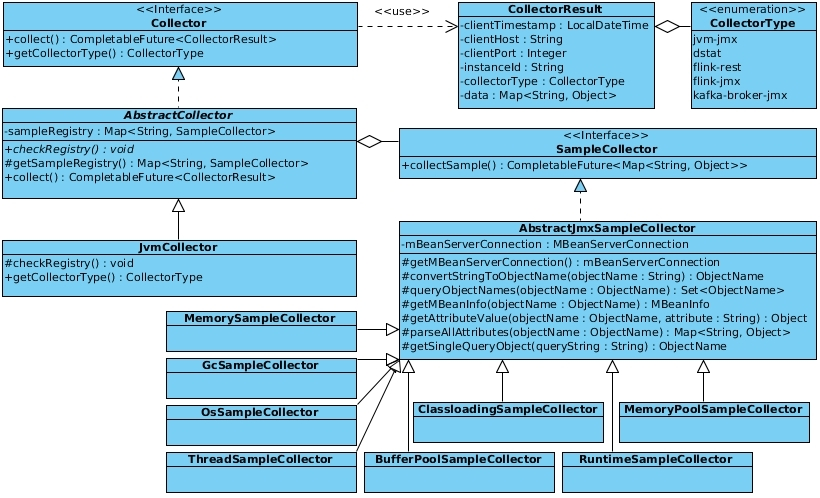
\includegraphics[width=1.0\textwidth]{../uml/class-jvm-collector.jpg}
	\caption{Class diagram 'JvmCollector'}
	\label{class-diagram-jvm-collector}
\end{figure}

This overview describes the collector domain, that is equal to all implementations and consists of following parts:
\begin{enumerate}
    \item \verb|CollectorType|:
    Enumeration, meta information, that distinguishes collectors implementations
    \item \verb|CollectorResult|: Data container, the result of a single invocation of the collect() method from
    the Collector interface. Describes a data event, an immutable fact" at a given time, containing the host and port
    the client is running on, the type of collector and the requested data.
    \item \verb|Collector|: The main interface for implementations, defines the protocol for data collection.
    \item \verb|AbstractCollector|: Abstract class, provides the implementation of the main collect() method.
    \item \verb|SampleCollector|: An interface for all classes that collect samples defined by the group the data
    belongs to.
\end{enumerate}

On the example of \verb|JvmCollector|, the following section explains the basic design principles that is common
to the main collector domain more in detail wheras only relevant implementation details will be discussed in
subsequent implementations, because the process of collecting data is similar in all.

\subsection{JvmCollector}
\label{subsec:impl-jvmcollector}

The implementation of the \verb|Collector| interface for fetching "default" JVM data according to \autoref{tbl:jmxjvmdata}.
This basic set of different management interfaces build the foundation
for the implementation for collecting JVM related data like memory, garbage collector or thread information.

To keep the main implementation as small as possible and following the "Separation Of Concerns" pronciple,
the data was divided into different "sample groups", which resulted in one implementation each for collecting
memory, garbage collector, thread data, et al.

A these \verb|SampleCollector| implementations provide a  \verb|collectSample()| method, that fetches data from a different data group, here
on the example of the class \verb|MemorySampleCollector|.

\begin{lstlisting}[caption={MemorySampleCollector collectSample()}, captionpos=b, label={lst:memory-sample-collect}]
private static final String OBJECT_NAME = "java.lang:type=Memory";

@Override
public CompletableFuture<Map<String, Object>> collectSample() {
    return CompletableFuture.supplyAsync(() -> {
        final Map<String, Object> memoryResultMap = Maps.newLinkedHashMap();
        memoryResultMap.put(SAMPLE_KEY, parseMemory(getMemoryMXBean(OBJECT_NAME)));
        return memoryResultMap;
    });
}

private Map<String, Object> parseMemory(final MemoryMXBean proxy) {
    final Map<String, Object> memoryDataMap = Maps.newLinkedHashMap();
    memoryDataMap.put(MEMORY_OPFC_KEY, proxy.getObjectPendingFinalizationCount());
    return memoryDataMap;
}

private MemoryMXBean getMemoryMXBean(final String objectName) {
    try {
        return ManagementFactory.newPlatformMXBeanProxy(mBeanServerConnection(), objectName, MemoryMXBean.class);
    } catch (IOException ex) {
        throw ex;
    }
}
\end{lstlisting}

As one of the non-functional requirements in \autoref{ch:requirements}, the client implementation may not cause a negative impact
on source systems regarding system resources like cpu or disk usage. To make the code as "non-blocking" as possible,
the implementation is based on the usage of the class \verb|CompletableFuture|. It models an asynchronous computation and provides
a reference to its results that will be available when the computation itself is completed. These computations like the JMX
access in the example above, are potentially time-consuming \cite{Java8}. The \verb|CompletableFuture| allows the caller thread to return immediately
to perform other operations instead of waiting for the result of the computation of JMX memory data, by delegating to a
separate thread performing the operations defined in the \verb|CompletableFuture|.

The code above wraps the computation of JMX memory data, which contains the data access via the MBeanServerConnection,
introduced in \autoref{ch:basic-concepts}, and the preparation of result data in a separate thread performing the operations defined
in the futures method body.

The implementations for the other \verb|SampleCollector|s are almost the same, it only differs in the JMX management bean the data will
be queried from.

Every \verb|Collector| implementation is based on an internal registry of \verb|SampleCollector|s, every implementation must provide its
own registry required for the main  \verb|Collector| process, that delegates to its registered \verb|SampleCollector|s,
aggregates their results and creates the overall result for the \verb|Collector|. To split the collection into individual sample groups has
the advantage, that it makes the implementation very flexible regarding the data to collect. To add further data sources, it
will be enough to provide an implementation of the \verb|SampleCollector| interface and to add an entry to the registry.

\begin{lstlisting}[caption={Sample registry for "JvmCollector"}, captionpos=b, label={lst:jvmsampleregistry}]
private static Map<String, SampleCollector> jvmSampleRegistry(final MBeanServerConnection mBeanServerConnection) {
    final Map<String, SampleCollector> registry = Maps.newHashMap();
    registry.put(MemorySampleCollector.SAMPLE_KEY, new MemorySampleCollector(mBeanServerConnection));
    registry.put(ThreadSampleCollector.SAMPLE_KEY, new ThreadSampleCollector(mBeanServerConnection));
    ...
    return registry;
}

@Override
public CollectorType getCollectorType() {
    return CollectorType.JVM_JMX;
}

@Override
protected void checkRegistry() {
    if (getSampleRegistry().isEmpty()) {
        throw new JmxCollectorException();
    }
}
\end{lstlisting}

The \verb|JvmCollector| implementation only provides the sample registry, the type of collector as well as a simple check if \verb|SampleCollector|s
are registered at all. These methods are defined in the \verb|AbstractCollector| class, discussed in the next section.

\subsection{AbstractCollector}

The abstract base class for all \verb|Collector| implementations that contains the registry of \verb|SampleCollector|s to be used in the main
collection process shown below.

\begin{lstlisting}[caption={"AbstractCollector" sample registry}, captionpos=b, label={lst:abstract-collectorsample-registry}]
private final Map<String, SampleCollector> sampleRegistry;
\end{lstlisting}

The collection process, defined by the \verb|collect()| method in the \verb|Collector| interface is implemented in this abstract class and
therefore the same for all implementations. The only requirement for implementing classes is to provide realizations for the abstract methods in this class.
The following steps are performed:
\begin{lstlisting}[caption={"AbstractCollector" Fetch sample futures}, captionpos=b, label={lst:abstract-collector-step-one}]
final List<CompletableFuture<Map<String, Object>>> sampleResultCPList = getSampleRegistry().values()
    .stream()
    .map(SampleCollector::collectSample)
    .collect(Collectors.toList());
\end{lstlisting}

This demonstrates the Stream features available since Java 8, that enable the processing of collections in a
more functional manner more focussed on the data transformations rather than the data itself. The
implementation creates a Stream of registered \verb|SampleCollector|s, collect the data for each sample and create a list of containing
futures, regarding to to \verb|SampleCollector| interface.

To merge the computations from multiple \verb|SampleCollector|s and extract the the data from \verb|CompletableFuture|s:

\begin{lstlisting}[caption={"AbstractCollector" Merge and extract data }, captionpos=b, label={lst:abstract-collector-step-two}]
final List<Map<String,Object>> sampleResults =
    sampleResultCPList
        .stream()
        .map(CompletableFuture::join)
        .collect(Collectors.toList()))
\end{lstlisting}

\begin{lstlisting}[caption={"AbstractCollector" Create CollectorResult}, captionpos=b, label={lst:abstract-collector-step-three}]
final Map<String, Object> dataMap = Maps.newLinkedHashMap();
sampleResults.forEach(dataMap::putAll);
final CollectorResult collectorResult = new CollectorResult(getCollectorType().name().toLowerCase(),dataMap);
return collectorResult;
\end{lstlisting}

At the end, the \verb|CollectorResult| containing the type and the data will be generated.

The implementations discussed in coming sections are all based on the concept, to divide the collection into separate units and
to create an overall result by aggregating individual sample data. As a result of this approach, the implementations keeps flexible
what makes it easy to add or remove sample data just by providing implementations of the \verb|SampleCollector| interface or removing
an item from the internal registry. In addition, as shown above in the \verb|JvmCollector| class in \autoref{lst:jvmsampleregistry},
the collection of sample data and the
preparation of the \verb|CollectorResult| can be realized with just a few lines of code, which makes the integration of
further data sources quite easy. This will be demonstrated in the coming section.

\subsection{FlinkRestCollector}

This collector implementation fetches data from the HTTP monitoring API that comes with Apache Flink and uses the endpoints
introduced in \autoref{tbl:http-api-flink}.

\begin{figure}[H]
	\centering
	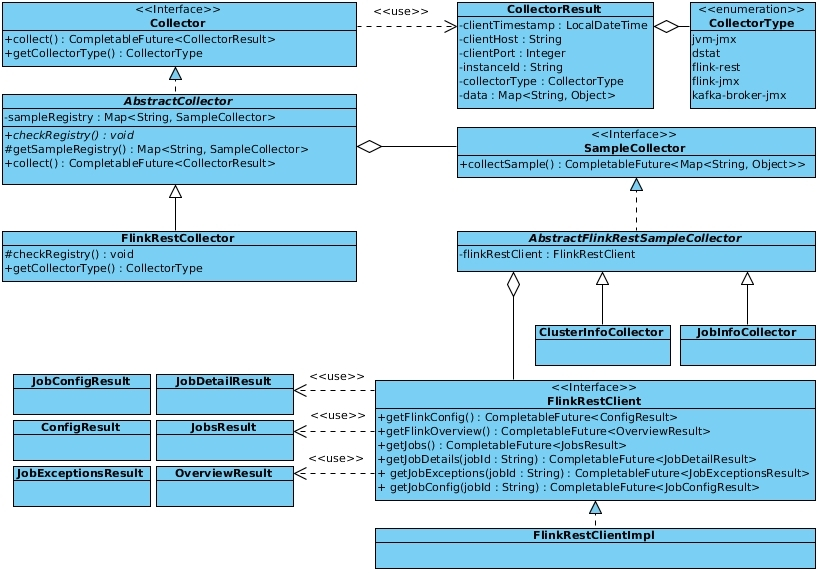
\includegraphics[width=1.0\textwidth]{../uml/class-flink-rest-collector.jpg}
	\caption{Class diagram 'FlinkRestCollector'}
	\label{class-diagram-flink-rest-collector}
\end{figure}

Following the sample approach described above, this \verb|Collector| implementation provides its internal sample registry,
containing the \verb|SampleCollector| implementations based on the data that is desired and shall be collected. Because the monitoring API provides data concerning
general server and cluster information as well as detailed information about jobs and their state, the registry contains
two appropriate \verb|SampleCollector|s:

\begin{lstlisting}[caption={"FlinkRestCollector" Sample registry}, captionpos=b, label={lst:flink-rest-collector-sample-registry}]
private static Map<String, SampleCollector> flinkRestSampleRegistry(final FlinkRestClient flinkRestClient) {
    final Map<String, SampleCollector> registry = Maps.newHashMap();
    registry.put(ClusterInfoCollector.SAMPLE_KEY, new ClusterInfoCollector(flinkRestClient));
    registry.put(JobInfoCollector.SAMPLE_KEY, new JobInfoCollector(flinkRestClient));
    return registry;
}
\end{lstlisting}

The implementation of \verb|SampleCollector| just differs in the way of data access. While the \verb|JvmCollector| uses an \verb|MBeanServerConnection|
to query data using the JMX management interface, \verb|FlinkRestCollector| is based on a REST client internally to request data, which builds
on the \verb|RestTemplate| class, provided by the Spring Framework:

\begin{lstlisting}[caption={"FlinkRestCollector" Rest client}, captionpos=b, label={lst:flink-rest-collector-client}]
final CompletableFuture<OverviewResult> flinkOverviewFuture = restClient().getFlinkOverview();
...
final Map<String, Object> dataMap = Maps.newLinkedHashMap();
dataMap.put(FLINK_JOBS_RUNNING_KEY, flinkOverview.getJobsRunning());
dataMap.put(FLINK_FINISHED_KEY, flinkOverview.getJobsFinished());
dataMap.put(FLINK_CANCELLED_KEY, flinkOverview.getJobsCancelled());
dataMap.put(FLINK_FAILED_KEY, flinkOverview.getJobsFailed());
final Map<String, Object> resultMap = Maps.newLinkedHashMap();
resultMap.put(SAMPLE_KEY, dataMap);
return resultMap;
\end{lstlisting}

By providing this sample data, this \verb|Collector| creates a \verb|CollectorResult| containing the data fetched from Apache Flinks monitoring
API without the need to change the main collector process.

\subsection{DStatCollector}

To collect system related data defined in \autoref{tbl:dstatcategories}, this implementation uses the Dstat system tool,
that provides multiple parameters to specify the data to be displayed. According to the data analysis, following parameters will be used:

\begin{lstlisting}[caption={"DstatCollector" program parameters in }, captionpos=b, label={lst:dstat-parameters}]
private static final String[] DSTAT_COMMAND = {"dstat", "-t",
    "--cpu", "--top-cpu-adv", "--top-cputime", "--top-cputime-avg",
    "--disk", "--disk-tps", "--disk-util",
    "--net", "--socket", "--tcp", "--udp",
    "--io", "--top-io-adv", "--lock", "--fs",
    "--mem", "--top-mem", "--page", "--swap", "--vm",
    "--sys", "--load", "--ipc", "--unix",
    "--proc", "--proc-count", "--top-latency", "--top-latency-avg",
    "--full",
    "--float", "1", "0"};
\end{lstlisting}

According to the given parameters, the \verb|DstatCollector| class is based on the implementations for \verb|CpuSampleCollector|,
\verb|DiskSampleColletor|, etc., which will have to be registrered using a sample registry, as discussed in the sections above.

Starting the Dstat process with the given parameters results in string containing three lines, where only the third line ist required to
to gather data of. To start the external process and to retrieve the resulting output, a \verb|ProcessBuilder| is used, which is part of
the java.lang package.
\begin{lstlisting}[caption={ProcessBuilder in "DstatCollector"}, captionpos=b, label={lst:dstatprocessbuilder}]
final ProcessBuilder processBuilder = new ProcessBuilder(DSTAT_COMMAND);
processBuilder.redirectErrorStream(true);
final Process process = processBuilder.start();
try (BufferedReader processOutputReader =
    new BufferedReader(new InputStreamReader(process.getInputStream()))) {
        final String dstatResult = processOutputReader.lines()
            .map(String::toString)
            .collect(Collectors.joining(System.lineSeparator()));
        final int exitCode = process.waitFor();
}
\end{lstlisting}

All Dstat sample collectors are based on regular expressions, the third line of the result is splitted, and the data of interest
extracted:
\begin{lstlisting}[caption={"CpuSampleCollector", Extract sample data}, captionpos=b, label={lst:cpusamplecollector}]
final Pattern CPU_USAGE_PATTERN = Pattern.compile("" +
    "(\\d+(\\.\\d+)?)(\\s*)" +
    "(\\d+(\\.\\d+)?)(\\s*)" +
    "(\\d+(\\.\\d+)?)(\\s*)" +
    "(\\d+(\\.\\d+)?)(\\s*)" +
    "(\\d+(\\.\\d+)?)(\\s*)" +
    "(\\d+(\\.\\d+)?)")
...
final Matcher matcher = CPU_USAGE_PATTERN.matcher(raw.trim());
final Map<String, Object> cpuUsageMap = Maps.newLinkedHashMap();
if (!matcher.matches()) {
    LOG.warn("Unable to parse 'CpuUsage'");
} else {
    try {
        cpuUsageMap.put(CPU_NAME_KEY, cpuName);
        cpuUsageMap.put(CPU_USAGE_USER_KEY, Float.valueOf(matcher.group(1)));
        cpuUsageMap.put(CPU_USAGE_SYSTEM_KEY, Float.valueOf(matcher.group(4)));
        ...
        } catch (NumberFormatException ex) {
            LOG.warn("Unable to parse 'CpuUsage'");
        }
}
\end{lstlisting}

\subsection{FlinkJmxCollector and KafkaBrokerJmxCollector}

The collection of application data using JMX for Apache Flink and Apache Kafka is working in the
same way as discussed in the previous sections. The implementations both provide \verb|SampleCollector|s for collecting data
from the managed resources which are listed for Apache Kafka in Appendix A by using a \verb|MBeanServerConnection| and querying the resources by their JMX ObjectName,
see \autoref{ch:basic-concepts}. Since Apache Flink is just providing a very basic set
of application data in its current version, containing rudimentary JVM data like cpu load and basic information about current
jobs and their state, this data will be collected nevertheless. It will be assumed to the metric system will be improved in upcoming versions
of Apache Flink. Furthermore the data is redundant, because the implementation of the \verb|JvmCollector| and \verb|FlinkRestCollector| provides a
more detailed set of JVM and job data.

\section{CollectorClient}
\label{sec:impl-collector-client}

After discussing the \verb|Collector| implementations in the previous section, this section introduces the \verb|CollectorClient|,
the core software component representing the entry point for bringing data into the system. This is the component that needs be
installed on Apache Flink and Apache Kafka source systems and has the following responsibilities:

\begin{enumerate}
    \item Register itself on application start with client-discovery
    \item Provide metadata for the \verb|CollectorManager| component available via REST resource
    \item Provide an interface to trigger data collection "on demand" from the \verb|CollectorManager|s web UI
    \item The main collection process, based on registered \verb|collector| implementations
    \item Transport data to the message broker
\end{enumerate}

\begin{figure}[H]
	\centering
	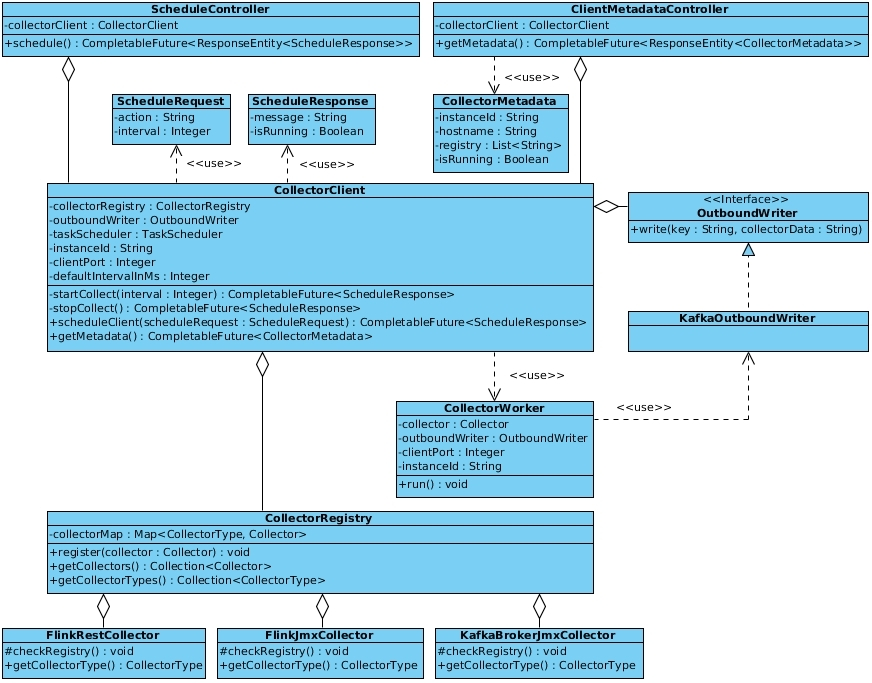
\includegraphics[width=1.0\textwidth]{../uml/class-collector-client.jpg}
	\caption{Class diagram 'CollectorClient'}
	\label{class-diagram-collector-client}
\end{figure}

The \verb|CollectorClient| is a small web service, a self-containing jar-file with an embedded Jetty servlet container realized using
Spring Boot. To register the client with the \textit{Consul Client-Registry}, Spring provides an annotation-based approach to accomplish
this functionality within spring-cloud sub-project, a set of tools for the development of cloud-based applications following common patters
of distributed systems like configuration management, cluster state, service-discovery, etc. .

\begin{lstlisting}[caption={"CollectorClientApp", Client registration}, captionpos=b, label={lst:collector-client-registration}]
@SpringBootApplication
@EnableDiscoveryClient
public class CollectorClientApp {

    public static void main(String[] args) {
        SpringApplication.run(CollectorClientApp.class, args);
    }
}
\end{lstlisting}

The \verb|@EnableDiscoveryClient| annotation seen above requires a Maven dependency to the \verb|spring-cloud-starter-consul-all| artefarct,
which provides and implementation to register the annotated Spring Boot application within the Consul service discovery. Based
on usefull default configurations, this application registers itself the default Consul host \verb|localhost| and port \verb|8500| and is
available to be discovered by the \verb|CollectorManager| component.

The \verb|CollectorClient| provides a Restful web service for fetching metadata for the respective client. This resource is required by
the \verb|CollectorManager| component for displaying detailed client data in the user interface.

\begin{lstlisting}[caption={"ClientMetadataController", Metadata REST endpoint}, captionpos=b, label={lst:metadata-endpoint}]
@Async
@RequestMapping(value="/client/metadata", method = RequestMethod.GET, produces = APPLICATION_JSON_VALUE)
public CompletableFuture<ResponseEntity<CollectorMetadata>> getMetadata() {
    LOG.debug("Entering getMetadata()");
    final CompletableFuture<ResponseEntity<CollectorMetadata>> responseCP = collectorClient.getMetadata()
        .thenApply(metadataMap -> {
            LOG.debug("Fetched client metadata: {}", metadataMap);
            return new ResponseEntity<>(metadataMap, HttpStatus.OK);
        });
        LOG.debug("Immediately return from getMetadata()");
        return responseCP;
    }
\end{lstlisting}

Both code snippets are a good examples for the "minimum of fuss" required to enable small web based services that registers itself
with a service-discovery server. In addition, the last snippet enables a REST resource, localized by the API
path \verb|/client/metadata|, listening for \verb|GET| requests and delivering metadata of the client in JSON format. Furthermore, the capabilities
of asynchronous computations is demonstrated, the \verb|@Async| annotation in combination with the future implementation as the return
value forces the framework to return immediately and not to block the caller thread, see \autoref{subsec:impl-jvmcollector}. Internally,
Spring Boot uses an \verb|ExecutorPool| for the execution of asyncronous computations in a different thread.

In analogy to the metadata enpoint seen above, the client realizes a uniform REST interface that enables the scheduling
of the data collection process. In this case, the servive expects \verb|POST| requests, that contain a \verb|ScheduleRequest| in their
request body provided by the clients that use this service. This body must be JSON formatted and contains the action to
trigger(start/stop data collection) and the time intervall between each collection process, five seconds for example. As result,
a JSON response will be returned, containg a status of the schedule request and the status of the \verb|CollectorClient| (running/stopped).

\begin{lstlisting}[caption={"ScheduleController", REST endpoint}, captionpos=b, label={lst:schedule-endpoint}]
@RequestMapping(value = "/client/schedule", method = RequestMethod.POST, consumes = APPLICATION_JSON_VALUE)
public CompletableFuture<ResponseEntity<ScheduleResponse>> schedule(@RequestBody @Valid final ScheduleRequest request,
    final BindingResult errors) {
LOG.debug("Received schedule request, action={}, interval={}", request.getAction(), request.getInterval());
    if (errors.hasErrors()) {
        throw new CollectorClientException("Invalid schedule request");
    }
    return collectorClient.scheduleClient(request)
        .thenApply(collectorScheduleResponse ->
            new ResponseEntity<>(collectorScheduleResponse, HttpStatus.OK));
}
\end{lstlisting}

Whereas the REST services seen above just take HTTP requests, the \verb|CollectorClient| contains the implementation for
collecting the data based on the concept of a registry of \verb|Collector|s. In contrast to the sample registry explained in the
\verb|Collector| implementations above, the registry holds the \verb|Collector|r implementations, and not any \verb|SampleCollector| which
are part of the \verb|Collector|s. The decoupling of \verb|Collector| implementations from the \verb|CollectorClient| by using a dynamic registry
allows to add further \verb|Collector|s and to remove existing ones without changing the \verb|CollectorClient| implementation.

The scheduling of the client uses Spring's \verb|TaskScheduler| interface that abstracts the scheduling of tasks based on different
kinds of triggers, where a task is an implementation of the \verb|Runnable| interface, defined in the Java core package \verb|java.lang.thread|.
Based on a Stream of registred \verb|Collector| implementations, the client creates instances of the \verb|CollectorWorker| class, that
encapsulates the collection process for execution in a separate thread which will be provided to the task \verb|TaskScheduler|.

\begin{lstlisting}[caption={"CollectorClient", collector registry}, captionpos=b, label={lst:collector-client-registry}]
private List<ScheduledFuture<?>> collectorTaskFutures = null;
...
collectorTaskFutures = collectorRegistry.getCollectors()
    .stream()
    .map(collector -> new CollectorWorker(collector, clientPort, outboundWriter, instanceId))
    .map(collectorWorker -> taskScheduler.scheduleWithFixedDelay(collectorWorker, interval))
    .collect(Collectors.toList());
\end{lstlisting}

The \verb|CollectorWorker| implements \verb|Runnable| interface, hence it must provide an implementation of the parameter-less
\verb|run()|-method. Within its implementation, it fetches the \verb|CompletableFuture| containing collected data, creates a \verb|CollectorResult|
and enriches it with client information, that makes the data set uniquely identifiable.

\begin{lstlisting}[caption={"CollectorWorker", collector registry}, captionpos=b, label={lst:collector-worker}]
private final Collector collector;
private final OutboundWriter outboundWriter;
...
@Override
public void run() {
    LOG.debug("Collector worker starts...");
    collector.collect()
        .thenAccept(collectorResult -> {
            try {
                final CollectorResult result = new CollectorResult(collectorResult.getCollectorType(),
                    collectorResult.getData(), now(), InetAddress.getLocalHost().getHostAddress(),
                                clientPort, instanceId);
                final String jsonData = JsonUtils.toJson(result);
                outboundWriter.write(collector.getCollectorType().name().toLowerCase(), jsonData);
            } catch (UnknownHostException ex) {
                throw new CollectorClientException(ex.getMessage());
            }
    });
    LOG.debug("Collector worker finished");
}
\end{lstlisting}

After the result is created, it will be transfered into its JSON representation and written into a Apache Kafka topic, by using
the \verb|OutboundWriter| interface, whose implementation \verb|KafkaOutboundWriter| uses the class \verb|KafkaTemplate|, provided by the Spring sub-project spring-kafka.

\begin{lstlisting}[caption={"KafkaOutboundWriter", Send data}, captionpos=b, label={lst:outbound-writer}]
private final KafkaTemplate<String, String> kafkaTemplate;
private final String kafkaOutboundTopic;
...
@Override
public void write(final String key, final String jsonData) {
    LOG.debug("Trying to send data to Kafka");
    final ListenableFuture<SendResult<String, String>> sendResultFuture =
        kafkaTemplate.send(kafkaOutboundTopic, key, jsonData);
    sendResultFuture.addCallback(new ListenableFutureCallback<SendResult<String, String>>() {
        @Override
        public void onSuccess(final SendResult<String, String> response) {
                LOG.debug("Successfully send data to Kafka, topic={}, key={}", kafkaOutboundTopic, key);
        }

        @Override
        public void onFailure(final Throwable ex) {
            final OutboundWriterException exception = new OutboundWriterException(format("Error sending data to Kafka: %s", ex.getMessage()));
            LOG.warn(exception.getMessage());
            throw exception;
        }
    });
}
\end{lstlisting}
At this point, the collection process is finished. After the collection interval elapsed, which is configured to be five seconds as
default value, everything will be triggerd again by the \verb|TaskScheduler| described above.

\section{CollectorManager}

The \verb|CollectorManager| is a small web appliction representing the management component in the \textit{"Collector-Platform"}, it
realizes a basic HTML based user interface and provides an overview of all clients registred in the platform as well as a
detailed view of individual clients. In addition, the data collection process can be triggered by using this interface.

\begin{figure}[H]
	\centering
	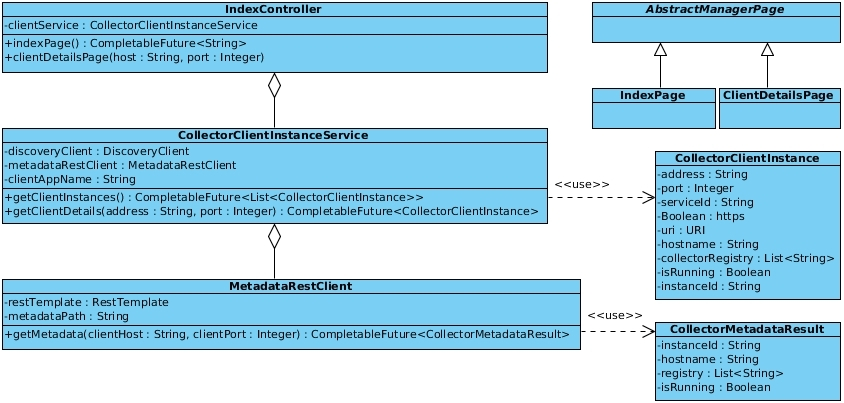
\includegraphics[width=1.0\textwidth]{../uml/class-collector-manager.jpg}
	\caption{Class diagram 'CollectorManager'}
	\label{class-diagram-collector-manager}
\end{figure}

To retrieve the required information of which clients exist and are registered in the system platform, the \verb|CollectorManager|
uses the \verb|DiscoveryClient| implementation provided by spring-cloud.

\begin{lstlisting}[caption={"CollectorClientInstanceService", Get client instances}, captionpos=b, label={lst:client-instance-service}]
private final DiscoveryClient discoveryClient;
private MetadataRestClient metadataRestClient;
...
final List<CollectorClientInstance> clients = discoveryClient.getInstances(clientAppName)
    .stream()
    .map(serviceInstance ->
        CollectorClientInstance.of(serviceInstance.getHost(), serviceInstance.getPort(), serviceInstance.getServiceId(),
        serviceInstance.isSecure(), serviceInstance.getUri())).collect(Collectors.toList());
        LOG.debug("Fetched all client instances: {}", clients);
        return clients;
\end{lstlisting}

The \verb|DiscoveryClient| provides access to the Consul Client-Registry and makes a list of all registered \verb|CollectorClient|s
available that will be displayed in the user interface. In addition, it sends a REST request to the \verb|CollectorClient| itself to enrich
existing Consul data with metadata provided by client as seen in the \verb|CollectorClient| implementation above.

\section{Summary}

The last chapter discussed implementation details for existing data collectors available for Apache Flink and and Apache Kafka.
It introduced the concept of a "sample registry", that divides the main data collection into separate units of work, represented
by implementations of the \verb|SampleCollector| interface. The "main" collectors, means classes that implement the \verb|Collector|
interface, aggregate an overall result based on individual data from multiple \verb|SampleCollector|s.

The \verb|CollectorClient| is based on implementations of the \verb|Collector| interface, which are also organized by an internal registry.
It represents a small REST-based web service that manages the collection process based on registered \verb|Collector|s and provides a REST
interface to enable the collection of data "on-demand".

The \verb|CollectorManager| acts a client for the web services provided by the \verb|CollectorClient|. It uses the REST resources discussed
for listing registered clients, showing detailed client information and starting and stopping the collection process in a basic
HTML-based user interface.

Wheras the \verb|Collector| implementations do not depend on Spring Boot, the framework is used to realize the \verb|CollectorClient| and
\verb|CollectorManager| applications. It enables the development of standalone, self-contained applications with less efford and makes
the integration of 3rd party applications or frameworks, in this example Apache Kafka and Consul, very easy.

The next chapter introduces the local test environment and explains the setup of the prototype application to enable the
evaluation of the software solution according to the requirements defined in \autoref{ch:requirements}.